%****************************************************************
\chapter{Flow Export Protocols}\label{ch:flow-export-protocols}
%****************************************************************

\section{NetFlow}\label{sec:netflow}
NetFlow \cite{rfc3954} by Cisco Systems is a protocol that allows network elements to export \ac{IP} flow information to designated collectors from where they can be later retrieved for further analyses. The collected flow-records are flexible enough to be used for a variety of purposes such as billing and mediation, network and user monitoring, resource provisioning, security analysis and data mining research works.  

\lstset{caption=A Flow Example, 
				tabsize=2, language=C, numbers=left,stepnumber=1,
				numberstyle=\ttfamily\color{gray}, keywordstyle=\color{blue},
				frame=shadowbox, rulesepcolor=\color{black}, 	
			  label=lst:flow-example, aboveskip=20pt, captionpos=b}
\begin{lstlisting}
(A) --> [SYN] ------>(B)
(A) <-- [SYN/ACK] <--(B)
(A) --> [ACK] ------>(B)
\end{lstlisting}
A flow is defined by a $7$-tuple flow-key, namely: \texttt{\{srcIP}, \texttt{dstIP}, \texttt{srcPort}, \texttt{dstPort}, \texttt{ipProto}, \texttt{ifIndex}, \texttt{ipTOS\}}. \ac{IP} packets with identical flow-keys become part of one flow. Two flows resulting from a three-way \ac{TCP} handshake for \marginpar{what is a flow?} example are shown in listing \ref{lst:flow-example}. In addition to the flow-key, flow-records can also contain additional accounting information such as flow start and end times, number of packets/octets in a flow, source/destination \ac{AS} numbers, et al.

\begin{figure}[h!]
\begin{center}
  \includegraphics* [width=0.7\linewidth]{figures/netflow-overview}	
  \caption{NetFlow: Overview \cite{nmelnikov:thesis:2010}}
  \label{fig:netflow-overview}
\end{center}
\end{figure}
A high-level abstracted functioning of NetFlow is shown in figure $\ref{fig:netflow-overview}$. The flow exporter reads the \ac{IP} packets that cross its boundary to generate flow-records. The flow-records are exported based on some predefined expiration rules, such as a \ac{TCP} \texttt{FIN} or \texttt{RST}, an inactivity timeout, a regular export timeout or crossing a low memory threshold. To achieve efficiency when handling large amounts of traffic, the flow-records are encapsulated in \ac{UDP} datagrams \marginpar{protocol operation} and are deleted from the exporter once transmitted. On the other end, the collector on receiving these flow-records, decodes and stores them locally to be used for further processing. 

The NetFlow version history is summarized in table $\ref{tab:netflow-versions}$. NetFlow v$1$ was introduced in the $90$s, however it was only until v$5$ with the introduction of \ac{CIDR} and \ac{AS} support that the \marginpar{version history} technology got mainstream. Today, NetFlow v$9$ is the de-facto industry standard and is the bases for \ac{IETF}'s \ac{IPFIX} effort to create a universal specification for \ac{IP} flow-export. 
\begin{table}[h!]
	\begin{center}
		\begin{tabular}{|c|c|}
			\hline	
			version & features \\
			\hline
			\hline 
			v$1, \{2,3,4\}$ & original format with several internal releases \\
			\hline 
			v$5$ & \ac{CIDR}, \ac{AS} support and flow sequence numbers \\
			\hline
			v$\{6,7,8\}$ & router-based aggregation support \\
			\hline
			v$9$ & template-based with \ac{IP}v$6$, and \ac{MPLS} support \\
			\hline
			\ac{IPFIX} & universal standard, transport-protocol agnostic\\
			\hline
		\end{tabular}
	\end{center}
	\caption{NetFlow Version History}
\label{tab:netflow-versions}
\end{table}

NetFlow v$9$ introduces templates in its export format. With templates, the exporter only needs to send required fields to the flow collector thereby reducing the volume of flow-data exported. In addition, fields can be added/removed from the flows without changing the export format. The transmission \marginpar{netflow v$9$} of records encapsulated in \ac{UDP} datagrams can lead to loss of flows when the link is congested and therefore the exporter and collector have usually been restricted to one-hop away dedicated links. To overcome this limitation, NetFlow v$9$ introduces transport support over congestion-aware \ac{SCTP}. In addition, NetFlow v$9$ also provides support for \ac{MPLS} and \ac{IP}v$6$ addresses. 

The ever increasing traffic volume crossing high-speed links, has been creating an enormous pressure on the routers that also engaged in NetFlow export. Sampled NetFlow was thus introduced by Cisco Systems as an extension to NetFlow v$9$ \marginpar{sampled netflow} to tone down the gigantic computation, by allowing the routers to skip over to every $n^{th}$ packet for flow export. The sampling rate $(n)$ is indicated in the export header and is either configured or randomly selected. 

Though sampled NetFlow does a good job in reducing the exported traffic volume, the sampling rate is still static which either reduces accuracy at low traffic volumes or increases memory use at high traffic volumes. An adaptive algorithm introduced in \cite{cestan:2004} helps overcome this difficulty. The introduced renormalization technique helps guarantee that the sampling rate can not only adjust to variable traffic mixes but also to network congestion. It also ensures that the flow records do not span over measurement bins to be able to guarantee statistical accuracy. The authors claim, that \marginpar{adaptive netflow} these updates are easily deployable to any NetFlow v$9$ router through a software update. In addition they say, a simple hardware add-on (flow counting extension), can also add capability to accurately count non-\ac{TCP} flows, a feature long waiting to be seen in NetFlow v$9$.

Flexible NetFlow is the newest version of NetFlow v$9$ that incorporates \ac{PSAMP} \cite{rfc5474} ideas to be able to select individual packets and export them in a packet record. The packet selection can be either deterministic or random depending on the chosen filters and sampling mechanism \cite{rfc5475}. The exported packet records can even be authenticated and encrypted using either \ac{TLS} \cite{rfc5246} or \ac{DTLS} \cite{rfc4347} \marginpar{flexible netflow} to prevent data manipulation across the route. Since \ac{PSAMP} is based on \ac{IPFIX} \cite{rfc5476}, only its limited feature set is currently supported by Flexible NetFlow. Additional features include ability to custom define flow-keys and flow-expiration rules to drastically reduce the amount of content exported by restricting it to only the needed flow-fields, and additional flows with immediate and permanent caches to suit the export timings to specific needs.

The challenge to identify relevant records in gigantic collected datasets have fumed recent independent studies to discover flow dependencies. For instance, the authors in \cite{swang:2010}, describe a model that uses flow timing information by extending \marginpar{flowrank} the PageRank \cite{lpage:1999} algorithm to rank and thereby extract the most relevant flows. Their model is weighted using parameters like the amount of bandwidth consumed and the likehood of security threat a flow might result in.

Today, as the industry is moving towards data center virtualization, it has become inherently critical to obtain insights into the data center network behavior for optimizations and resource provisioning. Since, Flexible NetFlow's visibility is limited to the \ac{IP} protocol it currently cannot be used to monitor data-center traffic. NetFlow-lite was thus introduced by Cisco Systems, to flows at the layer $2/3$ level to increase data center visibility. NetFlow-lite \marginpar{netflow-lite} uses similar packet sampling mechanisms as introduced in Sampled NetFlow along with the combined flexibility of Flexible NetFlow v$9$ at the switch level. NetFlow-lite captures the layer $2$ traffic, encapsulates packet samples and pushes the NetFlow cache outside the switch into a element that can convert NetFlow-lite to Flexible NetFlow records. These flow-records are then later exported to legacy collectors from where they can be used for further processing. The authors in \cite{lderi:2011} provide the first implementation of NetFlow-Lite which works as an extension to nProbe \cite{lderi:2003} to seamlessly convert NetFlow-Lite records to NetFlow/\ac{IPFIX}.

\section{IPFIX}\label{sec:ipfix}
\ac{IPFIX} \cite{rfc5101} by \ac{IETF} is an interoperable protocol for \ac{IP} flow export. It is deemed to be the logical successor of Flexible NetFlow v$9$. The working group defines \ac{IPFIX} as, "a unidirectional, transport-independent protocol with flexible data representation and an information model covering most network management needs at layer $3$ and $4$". The \ac{PSAMP} working group \cite{rfc5476}, that defines standards to individually sample packets in a flow export using statistical methods has adopted \ac{IPFIX} as its underlying protocol for data transport.

\begin{figure}[h!]
\begin{center}
  \includegraphics* [width=0.7\linewidth]{figures/ipfix-overview}	
  \caption{IPFIX: Overview \cite{pkohler:2003}}
  \label{fig:ipfix-overview}
\end{center}
\end{figure}
The \ac{IPFIX} architecture is described in \cite{rfc5470} and is shown in figure \ref{fig:ipfix-overview}. The architecture consists of three elements: a meter, which generates flows from \ac{IP} packets, an exporter, which pushes these flows using \ac{IPFIX}, and \marginpar{architecture} a collector, that collects and saves these flows for offline storage. All these elements have a one-to-many relationship among them. The group is also working to define an intermediary element, that might work to either aggregate or anonymize the flows. 

\begin{figure}[ht]
	\begin{minipage}[b]{0.49\linewidth}
		\centering
		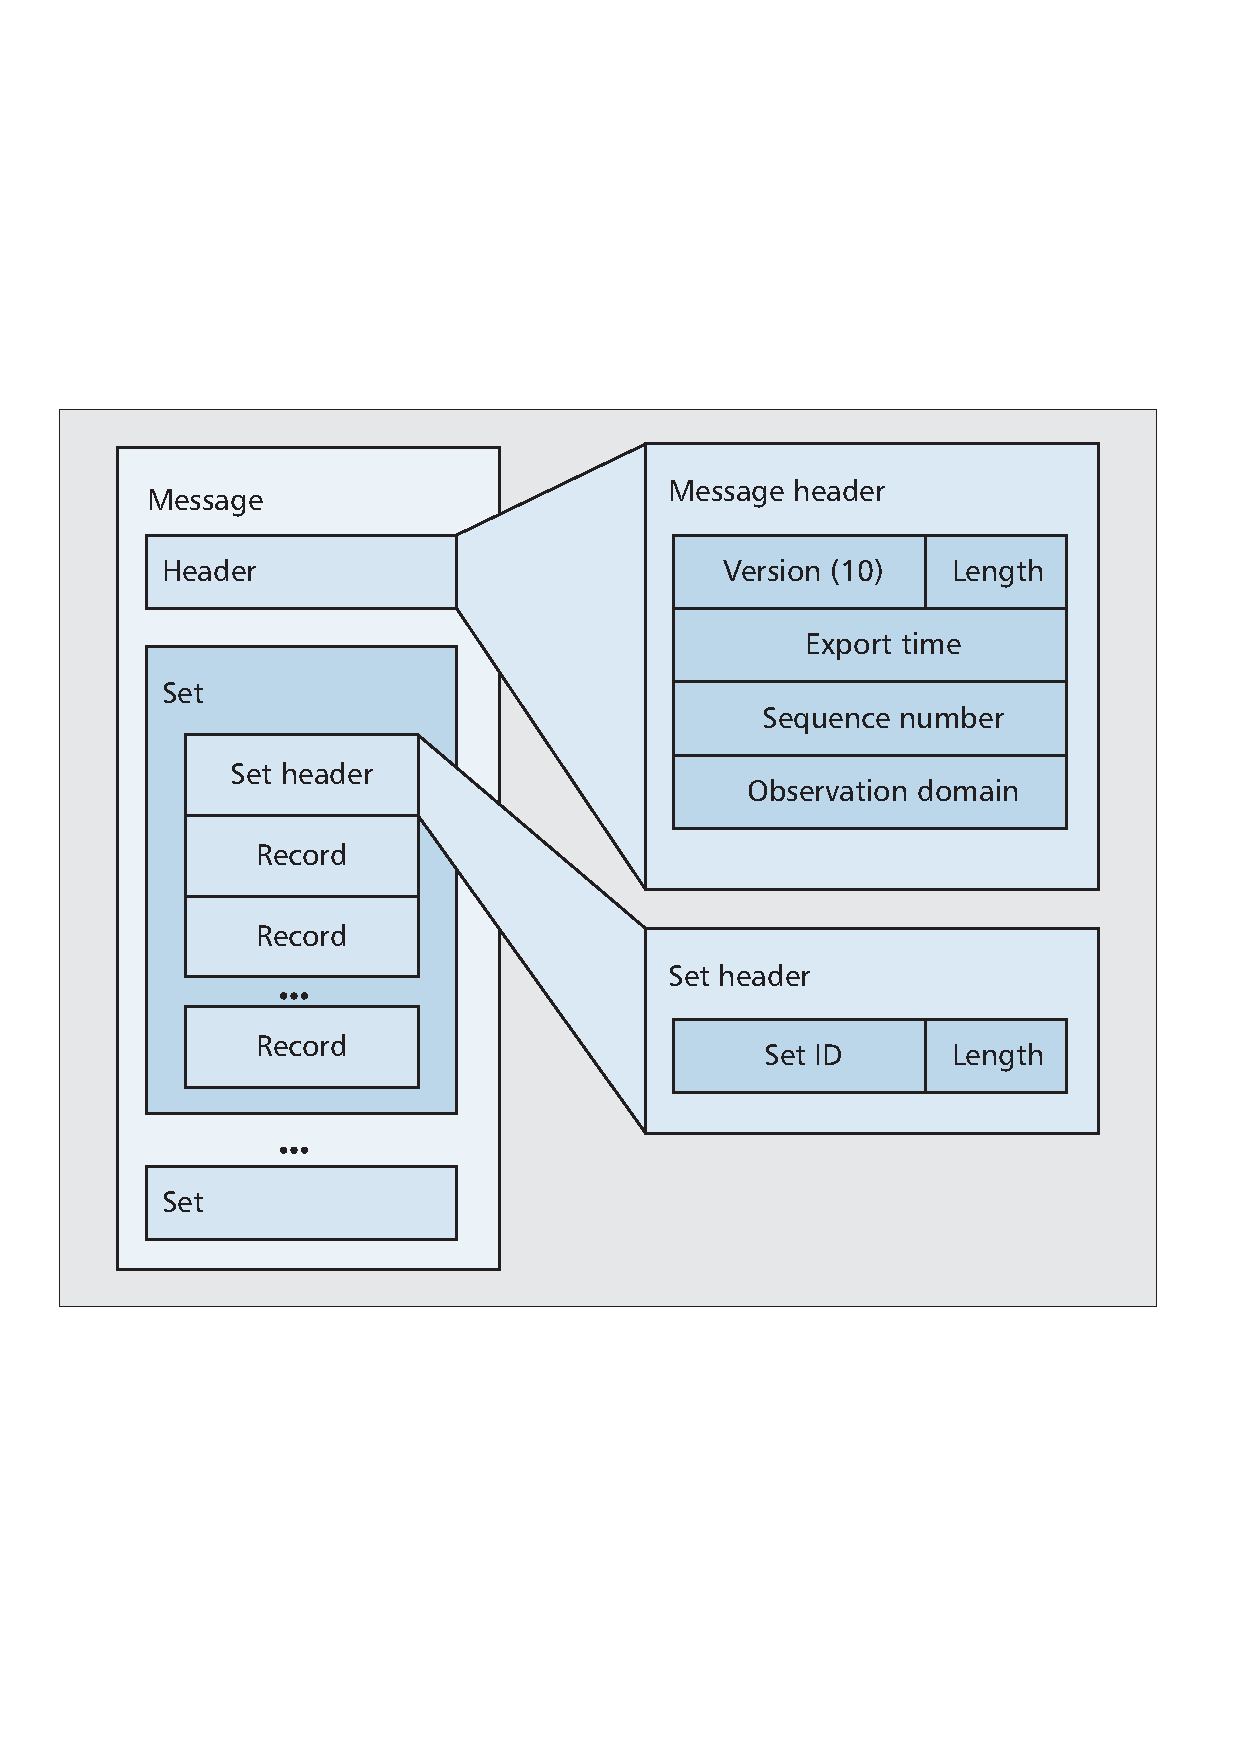
\includegraphics[width=0.7\linewidth]{figures/ipfix-message-structure}
		\caption{IPFIX: Messages \cite{btrammell:2011}}
		\label{fig:ipfix-message-structure}
	\end{minipage}	
	\begin{minipage}[b]{0.49\linewidth}
		\centering
		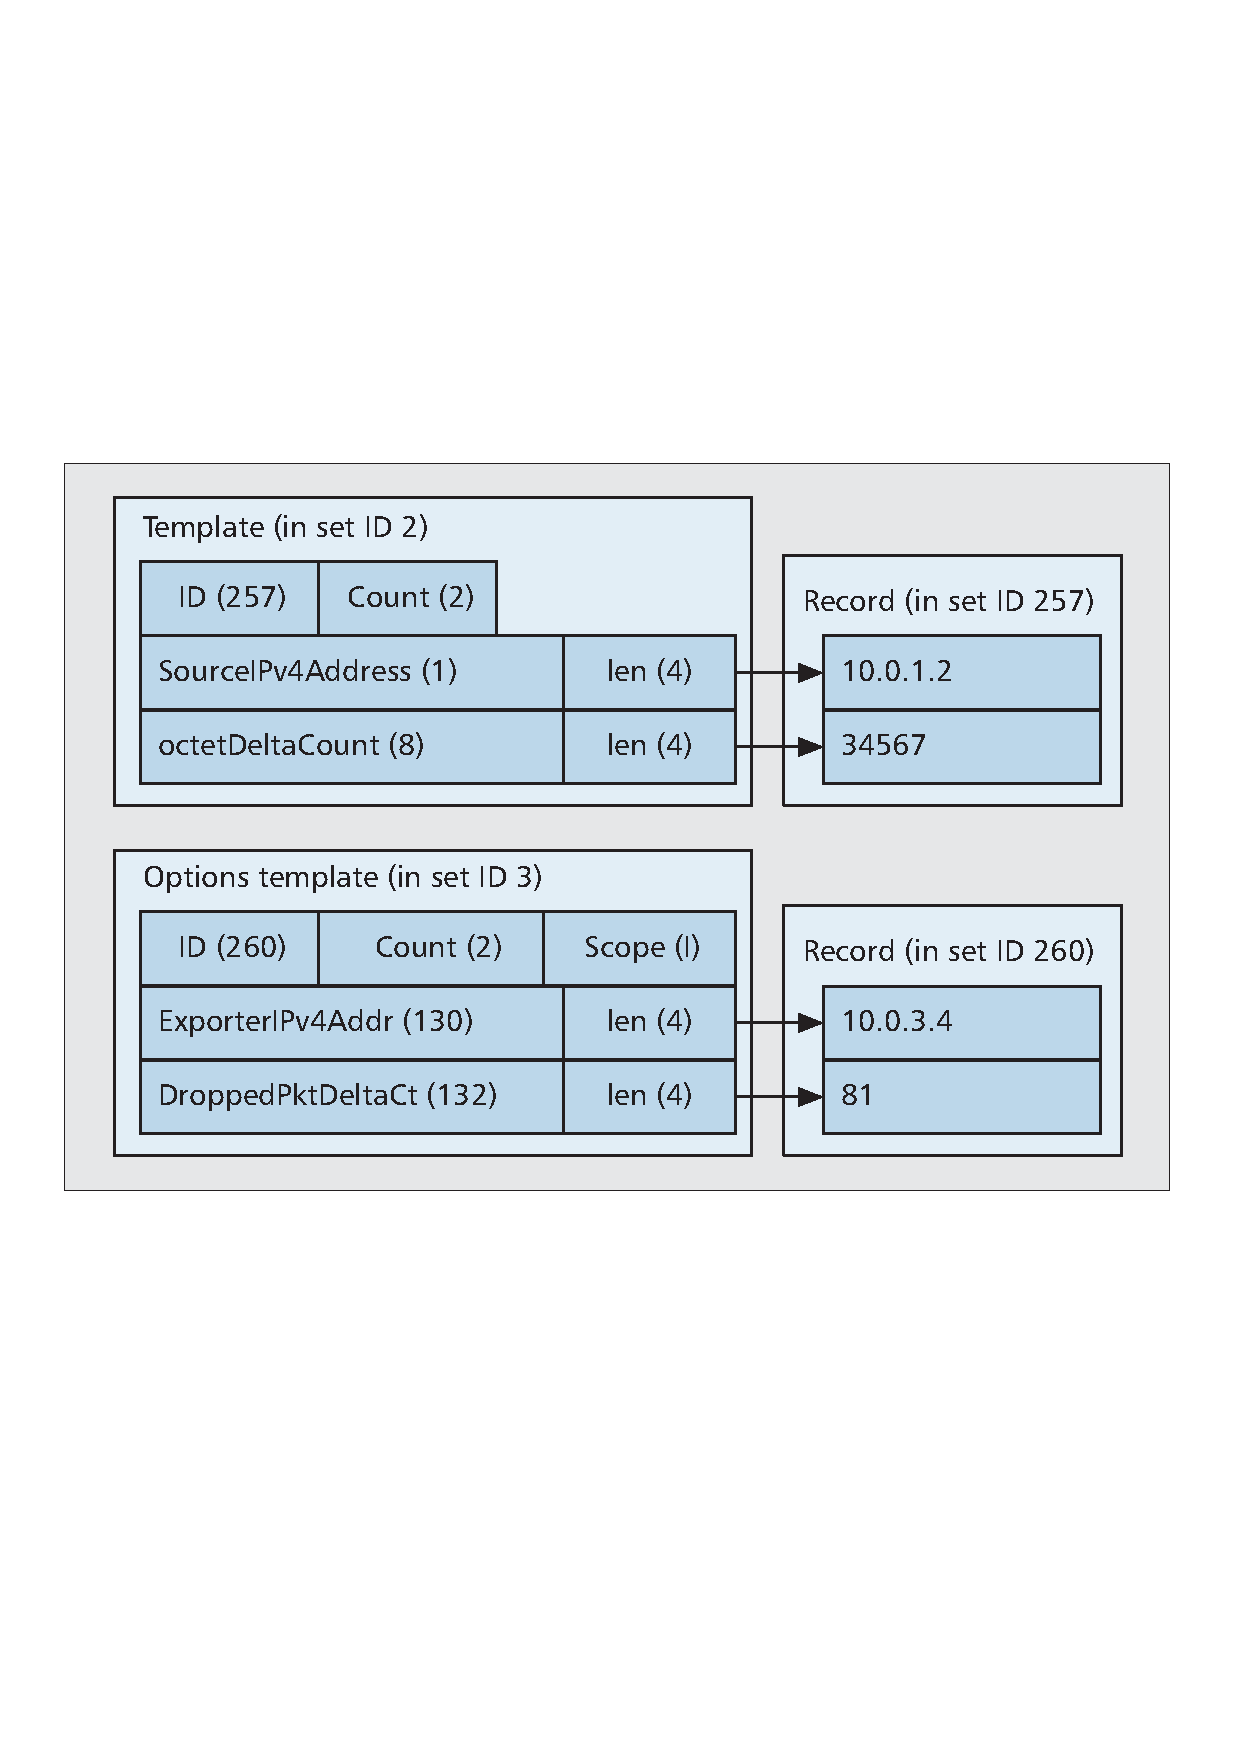
\includegraphics[width=0.7\linewidth]{figures/ipfix-information-element}
		\caption{IPFIX: Templates \cite{btrammell:2011}}
		\label{fig:ipfix-information-element}
	\end{minipage}	
\end{figure}
A message is a fundamental unit of data exchange in \ac{IPFIX}. Each such message consists of a $16$-byte header along with a number of sets as shown in figure $\ref{fig:ipfix-message-structure}$. A set can either be a template or a data set. Each such set in the message again contains a $16$-bit header and a number of records \marginpar{messages and templates} associated with it. Each record within a template set is a template that refers to a data record.  A template consists of a number of \ac{IE}s as shown in figure $\ref{fig:ipfix-information-element}$. These \ac{IE}s are encoded using reduced-length encoding scheme. \ac{IANA} keeps a registry \footnote{\url{http://www.iana.org/assignments/ipfix/ipfix.xml}} of all \ac{IE}s with a $16$-bit ID assigned to them. Templates can also contain enterprise-specific \ac{IE}s that are scoped using \ac{PENs} \footnote{\url{http://www.iana.org/assignments/enterprise-numbers}}. 

\begin{figure}[h!]
\begin{center}
  \includegraphics* [width=0.5\linewidth]{figures/ipfix-transport}	
  \caption{IPFIX: A Transport Session \cite{btrammell:2011}}
  \label{fig:ipfix-transport}
\end{center}
\end{figure}
An \ac{IPFIX} transport session is shown in figure $\ref{fig:ipfix-transport}$. It starts off with the \ac{EP} initiating a connection with the \ac{CP}. Once the connection is established, the \ac{EP} passes on the templates followed by the data that is described by them. These templates can later still be withdrawn by sending a control template of \ac{IE} count zero. The transport session can use either \ac{SCTP}, \ac{TCP} or \ac{UDP} as the \marginpar{transport and security} underlying protocol, although \ac{SCTP} is usually the preferred method given it allows selective reliability and congestion control. \ac{TCP} is supported to allow secure transport over \ac{TLS}, since \ac{DTLS} is only supported over \ac{UDP} and \ac{SCTP}. The connection-less behavior of \ac{UDP} calls for the template retransmission delay and template lifetime parameters to be exchanged between \ac{EP} and \ac{CP}. These transport sessions can also be stored in \ac{IPFIX} files and sent on top application layer protocols. 



\todo[inline]{IPFIX: Message Structure, Protocol Design, Future \ldots}

\section{sFlow}\label{sec:sflow}

\todo[inline]{sFlow: Start it! \ldots}